\section{Planteamiento del problema}
\label{ch:planteamiento}

\subsection{Antecedentes del problema}
\label{sec:antecedentes_problema}

Como ya se describió en el apartado anterior, la Mesa de Servicio del CCoE manejaba varios frentes de trabajo de forma simultánea: monitoreo de correos, seguimiento de páginas de clientes específicos y gestión de tickets en Zendesk. A esta carga se sumaba un número considerable de alertas activas generadas en AWS que aún no habían sido verificadas, ya que el proceso para revisarlas no estaba asignado a una persona en específico.

\subsection{Definición del problema}
\label{sec:definicion_problema}

La saturación de la Mesa de Servicio se reflejaba de forma concreta en el número de alertas activas sin verificar: se llegaron a registrar 129 alertas generadas en AWS pendientes de revisión (ver Figura \ref{fig:alertas_aws}).

\begin{figure}[h]
    \centering
    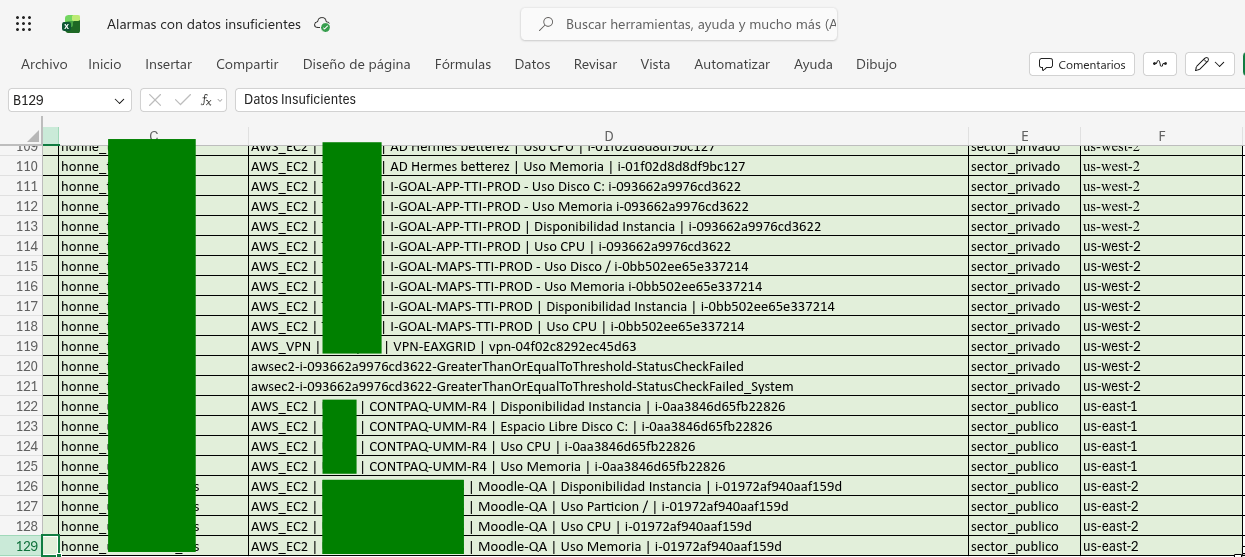
\includegraphics[width=0.8\textwidth]{img/figura_alertas_aws.png}
    \caption{Registro interno de alertas activas de AWS pendientes de verificación.}
    \label{fig:alertas_aws}
\end{figure}

Cada alerta debía revisarse manualmente para descartar falsos positivos, generados principalmente por dos causas: instancias que se apagaban de forma programada, lo cual generaba una alerta como si hubiera fallado aunque en realidad estaba funcionando como se esperaba; e instancias que ejecutaban tareas programadas, como respaldos, en horarios específicos, lo cual elevaba temporalmente el uso de CPU, disco, memoria o particiones hasta el 100\% y disparaba alertas de sobrecarga.

Aunque la verificación de alertas era responsabilidad de toda la Mesa de Servicio, no había una persona dedicada específicamente a esta tarea, por lo que las alertas reales y los falsos positivos se acumulaban en la misma bandeja, dificultando distinguir con rapidez cuáles requerían atención inmediata.

\subsection{Justificación}
\label{sec:justificacion}

Verificar cada alerta antes de reportarla era necesario porque Honne tiene la obligación contractual de informar a sus clientes sobre incidentes reales en sus instancias. Si un incidente real no se reportaba a tiempo, el cliente podía detectarlo por su cuenta y presentar una queja, lo cual representaba un riesgo de incumplimiento de contrato para la empresa. Al mismo tiempo, descartar los falsos positivos evitaba generar reportes innecesarios hacia clientes que no correspondían a una falla real.

Además, la incorporación de practicantes a esta tarea tenía como propósito liberar parte de la carga de trabajo de la Mesa de Servicio, distribuyendo la verificación de alertas para que el equipo pudiera enfocarse en la atención de incidentes reales y otras solicitudes.

\subsection{Objetivos}
\label{sec:objetivos}

\subsubsection{Objetivo general}
\label{subsec:objetivo_general}

Integrarse a la Mesa de Servicio del CCoE para apoyar en el uso de sus distintas herramientas de monitoreo y en el desarrollo de sus actividades diarias, contribuyendo a distribuir la carga de trabajo del área.

\subsubsection{Objetivos específicos}
\label{subsec:objetivos_especificos}

\begin{itemize}
    \item Verificar las alertas activas generadas en AWS, mediante las métricas de Amazon CloudWatch, para identificar falsos positivos y reportar los incidentes reales a los clientes correspondientes.
    \item Revisar los logs de instancias en Google Cloud Platform, mediante su consola de administración, para detectar problemas de latencia y errores recurrentes.
    \item Monitorear el estado de las soluciones y Agents de TIBCO Scribe (Scribesoft), revisando directamente los paneles de la plataforma, para verificar su disponibilidad.
    \item Desarrollar, en Python, un script de monitoreo automatizado que se conectara a TIBCO Scribe y notificara mediante un bot de Telegram cuando una solución presentara fallas recurrentes.
    \item Dar seguimiento a las alertas registradas en ServiceNow, mediante revisión constante de su bandeja, para notificar oportunamente al equipo responsable de su atención.
\end{itemize}

\subsection{Alcance y limitaciones}
\label{sec:alcance_limitaciones}

El apoyo brindado se centró en las herramientas de monitoreo utilizadas por la Mesa de Servicio del CCoE: alertas de AWS, logs de Google Cloud Platform, soluciones de TIBCO Scribe y alertas de ServiceNow, además del desarrollo de un script de automatización para una de ellas.

Como limitación, la función en todos los casos fue de detección y notificación, no de corrección directa de las fallas, ya que la resolución de incidentes correspondía a otras áreas, como SysAdmin. Tampoco se contó con un diagnóstico formal previo: las actividades fueron asignadas progresivamente por el asesor empresarial conforme surgían necesidades en el área.